\documentclass[11pt,a4paper]{article}

\usepackage{epsfig}
\usepackage{multicol}

\usepackage[utf8]{inputenc}
\usepackage[brazil]{babel}
\usepackage{fancyheadings}
\usepackage{amsmath}
\usepackage{calrsfs}
\usepackage{enumerate}
\usepackage{enumitem}   
\DeclareGraphicsExtensions{.png,.pdf}
\usepackage{amsmath, amsfonts, amssymb}
\usepackage{esint}
\usepackage{graphicx}
\usepackage{multicol}
\usepackage{tasks}
\usepackage[utf8]{inputenc}
\usepackage{mathrsfs} % Transformada de Laplace
\usepackage{indentfirst}
\usepackage{xcolor}

% As margens
\setlength{\textheight}{24.0cm}
\setlength{\textwidth}{17.5cm}
\setlength{\oddsidemargin}{2.0cm} % Margens reais desejadas
\setlength{\evensidemargin}{2.0cm} % 2+17.5+1.5=21cm (largura A4)
\setlength{\topmargin}{1.5cm} % 1.5+1.6+1.0+24.0+1.6=29.7cm
\setlength{\headheight}{1.6cm} % (altura A4)
\setlength{\headsep}{1.0cm}
\setlength{\columnsep}{1.5cm} % Coluna = 8cm ((17.5-1.5)/2)
\addtolength{\oddsidemargin}{-1in}
\addtolength{\evensidemargin}{-1in}
\addtolength{\topmargin}{-1in}
\setlength{\footskip}{0.0cm}


% Novos comandos
\newcommand{\limite}{\displaystyle\lim}
\newcommand{\integral}{\displaystyle\int}
\newcommand{\somatorio}{\displaystyle\sum}
\newcommand{\mat}[1]{\mbox{\boldmath{$#1$}}} 

\pagestyle{fancy}


\usepackage{lipsum}

\lhead{

\includegraphics[width=1cm]{brasao.png}
}

\rhead{ 
\sc\textbf{U}niversidade \textbf{F}ederal do \textbf{C}eará\\
Campus Quixadá\\ Lista 3 de Eletromagnetismo}

\cfoot{}

\begin{document}

	\begin{center}
		\Large Eletrostática - Potencial Elétrico. 
	\end{center}

\begin{flushleft}
\textbf{Nome:} Mateus Sousa Araújo. \\
\textbf{Matrícula:} 374858. \\
\textbf{Professor:} Antônio Joel Ramiro de Castro. \\
\textbf{Curso:} Engenharia de Computação. \\
\end{flushleft}

\begin{enumerate}

\item \textbf{Griffiths - Cap. 2 - Problema 2.25.}

Usando as equações $2.27$ e $2.30$, encontre o potencial a uma distância $z$ acima do centro das distribuições de carga da figura abaixo. Em cada caso, calcule $E = -\vec{\nabla} \ V$. Suponha que alteramos a carga do lado direito da Figura $a$ para $-q$; qual será, então, o potencial em $P$? Que campo isso sugere?

\begin{figure}[h]	
\centering % para centralizarmos a figura	
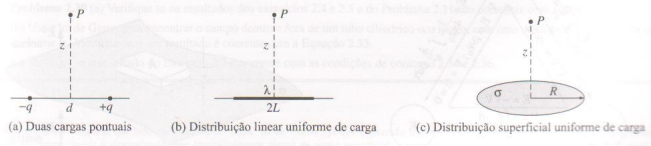
\includegraphics[width=13cm]{Selection_083.jpg} 
\caption{Distribuições de carga em diferentes configurações.}
\end{figure}


\textbf{RESOLUÇÃO}

\begin{enumerate}

\item 

Como temos uma distribuição discreta de cargas, então temos pelo princípio da superposição a seguinte relação:

$$V(r) = \displaystyle\dfrac{1}{4\pi\epsilon_0}\displaystyle\sum_{i=1}^n \displaystyle\dfrac{q_i}{r_i}$$

Somando a contribuição das duas cargas pela fórmula acima, chegamos em:
$$V(r) = \displaystyle\dfrac{1}{4\pi\epsilon_0} \displaystyle\dfrac{2q}{\sqrt{z^2 + (d/2)^2}}$$.

Fazendo $E = -\vec{\nabla} \ V$, temos:

$$E = \displaystyle\dfrac{1}{4\pi\epsilon_0} \displaystyle\dfrac{2qz}{\left(z^2 + (d/2)^2\right)^{3/2}} \mat{\hat{z}}$$.

\item

Como nesse caso temos uma distribuição contínua de cargas, temos a seguinte relação:

$$V(r) = \displaystyle\dfrac{1}{4\pi\epsilon_0}\displaystyle\int \displaystyle\dfrac{dq}{r}$$

Para a distribuição linear, temos:

$$V(r) = \displaystyle\dfrac{1}{4\pi\epsilon_0}\displaystyle\int_{-L}^{L} \displaystyle\dfrac{\lambda dx}{\sqrt{z^2 + x^2}} = \displaystyle\dfrac{1}{4\pi\epsilon_0} \ln(x + \sqrt{z^2 + x^2})|_{-L}^{L}$$

$$V(r) = \displaystyle\dfrac{\lambda}{4\pi\epsilon_0} \ln \left[ \displaystyle\dfrac{L + \sqrt{z^2 + L^2}}{-L + \sqrt{z^2 + L^2}}\right] = \displaystyle\dfrac{\lambda}{2\pi\epsilon_0} \ln \left( \displaystyle\dfrac{L + \sqrt{z^2 + L^2}}{z}\right).$$

Fazendo $E = -\vec{\nabla} \ V$, temos:

$$E = \displaystyle\dfrac{2L \lambda}{4\pi\epsilon_0} \displaystyle\dfrac{1}{z\sqrt{z^2 + L^2}} \mat{\hat{z}}$$.

Se fizermos a carga da direita ser $-q$ então o potencial no ponto desejado será $0$. Logo, isso também sugere que $E = -\vec{\nabla} \ V = 0$.

\item 

Como no item anterior, temos que assumir uma unidade infinitesimal de área e colocar na integral. Dessa forma, temos:

$$V(r) = \displaystyle\dfrac{1}{4\pi\epsilon_0}\displaystyle\int_{0}^{R} \displaystyle\dfrac{\sigma 2 \pi r dr}{\sqrt{r^2 + z^2}} = \displaystyle\dfrac{1}{4\pi\epsilon_0} 2 \pi \sigma (\sqrt{r^2 + z^2})|_{0}^{R}$$

$$V(r) = \displaystyle\dfrac{\sigma}{2\pi\epsilon_0} \left( \sqrt{R^2 + z^2} - z\right).$$

Fazendo $E = -\vec{\nabla} \ V$, temos:

$$E = \displaystyle\dfrac{\sigma}{2\pi\epsilon_0} \left[ 1 - \displaystyle\dfrac{z}{\sqrt{R^2 + z^2}}\right]\mat{\hat{z}}$$.

\end{enumerate}


\item \textbf{Griffiths - Cap. 2 - Problema 2.28.}

Use a equação $2.29$ para calcular o potencial dentro de uma esfera sólida de raio $R$ com densidade de carga uniforme e carga total $q$.

\textbf{RESOLUÇÃO}

Integrando em coordenadas esféricas, temos:

$$V(r) = \displaystyle\dfrac{\rho}{4\pi\epsilon_0} \displaystyle\int \displaystyle\dfrac{r^2 \sin \theta \ dr \ d\theta \ d\phi}{\sqrt{z^2 + r^2 - 2rz \cos \theta}}$$

$$\displaystyle\dfrac{\rho}{4\pi\epsilon_0}\displaystyle\int_0^\pi \displaystyle\dfrac{\sin \theta}{\sqrt{z^2 + r^2 - 2rz \cos \theta}} \ d\theta = \displaystyle\dfrac{1}{rz}(\sqrt{r^2 + z^2 - 2rz \cos \theta })|_{0}^{\pi} = \displaystyle\dfrac{1}{rz}(\sqrt{r^2 + z^2 + 2rz} - \sqrt{r^2 + z^2 - 2rz})$$

\item \textbf{Griffiths - Cap. 2 - Problema 2.29.}

Verifique se a Equação $2.29$ satisfaz a equação de Poisson, aplicando o laplaciano e usando a Equação $1.102$.

\textbf{RESOLUÇÃO}

$$\nabla^2V = \displaystyle\dfrac{1}{4\pi\epsilon_0} \ \nabla^2 \displaystyle\int \displaystyle\dfrac{\rho}{r} \ dr = \displaystyle\dfrac{1}{4\pi\epsilon_0} \displaystyle\int \rho(r') \left(\nabla^2 \displaystyle\dfrac{1}{r}\right) \ dr$$

Aplicando a propriedade da função Delta de Dirac temos:

$$\displaystyle\dfrac{1}{4\pi\epsilon_0} \displaystyle\int \rho(r') [-4\pi \delta^3(r - r')] \ dr = -\displaystyle\dfrac{1}{\epsilon_0} \rho(r).$$

Logo, a equação acima satisfaz a equação de Poisson.

\end{enumerate}
	
\end{document}